\documentclass[11pt]{article}

\usepackage[utf8]{inputenc}
\usepackage[T1]{fontenc}
\usepackage[french]{babel}
\usepackage[a4paper,margin=2.1cm]{geometry}
\usepackage{amsmath,amssymb}
\usepackage{graphicx}
\usepackage{booktabs}
\usepackage{float}
\usepackage{xcolor}
\usepackage{caption}
\usepackage{subcaption}  % charge caption automatiquement
\usepackage[colorlinks=true,linkcolor=blue!50!black,urlcolor=blue!50!black]{hyperref}
\captionsetup{font=small,labelfont=bf}

% Cherche les images que l'on compile depuis la racine du depot ou depuis rapports/
\graphicspath{{./}{../}}

\setlength{\parskip}{2pt}
\setlength{\parindent}{0pt}

% --------------------------------------------------------------------
\title{\vspace{-1.2cm}\textbf{De la classification des chiffres manuscrits\\
à la détection de cancers du sein}\\[2pt]
\large Une introduction aux réseaux de neurones convolutifs (CNN)\\[2pt]
\normalsize Projet de \emph{Mathématiques pour le Machine Learning} --- SM604\\
\normalsize Année 2025-2026, I1}

\author{\textbf{Équipe MML-MATH2-E}\\[2pt]
Eric Eung \quad Hugo Juzyna \quad Enzo Juzyna \quad Johnny Jin \quad James Him}

\date{7 juin 2026}
% --------------------------------------------------------------------

\begin{document}
\maketitle
\vspace{-0.6cm}

\begin{abstract}
\noindent Nous implémentons des réseaux de neurones pour trois problèmes de classification d'images
de difficulté croissante. \textbf{MNIST} compare un modèle linéaire et des MLP à une et deux couches
cachées (NumPy « à la main »), complétés par une étude du \emph{learning rate} ajoutée suite aux
conseils du professeur. \textbf{CIFAR-10} étend ces architectures aux images couleur et introduit un
CNN (PyTorch). \textbf{CBIS-DDSM} applique un CNN binaire à la détection de cancers du sein sur
mammographies réelles. Le fil conducteur est l'analyse critique : rôle du nombre de paramètres,
\emph{overfitting}, et surtout la mise en évidence puis la correction d'une \emph{fuite de données}
sur la partie médicale.
\end{abstract}

% ====================================================================
\section*{Prérequis --- Téléchargement des données (à lire avant exécution)}
% ====================================================================
\begin{center}
\fbox{\begin{minipage}{0.97\linewidth}\small
\textbf{\textcolor{red}{Le dataset CBIS-DDSM (images) n'est pas inclus dans le dépôt}} (volume trop
important). Pour exécuter la partie~3 (mammographies), téléchargez la version \textbf{JPEG} sur Kaggle :\\[2pt]
\url{https://www.kaggle.com/datasets/awsaf49/cbis-ddsm-breast-cancer-image-dataset/data?select=jpeg}\\[2pt]
puis placez le contenu dans le dossier \texttt{CBIS-DDSM/} en respectant l'arborescence
\texttt{CBIS-DDSM/archive/csv/} (fichiers \texttt{.csv}) et \texttt{CBIS-DDSM/archive/jpeg/} (images).
Un cache \texttt{.npy} est ensuite créé automatiquement au premier lancement. Les jeux \textbf{MNIST} et
\textbf{CIFAR-10} se téléchargent automatiquement (Keras / torchvision) : aucune action requise.
\end{minipage}}
\end{center}

\vspace{-0.1cm}
% ====================================================================
\section{MNIST --- Chiffres manuscrits}
% ====================================================================
\textbf{Données.} 70\,000 images $28\times28$ en niveaux de gris (60\,000 train / 10\,000 test).
Chaque image est aplatie en $\vec{x}\in\mathbb{R}^{784}$, normalisée dans $[0,1]$, et les étiquettes
$y\in\{0,\dots,9\}$ sont encodées en \emph{one-hot}.

\textbf{Modèles (NumPy).} (i) \emph{Linéaire} : $o=A\vec{x}+b$ puis \emph{softmax}. La combinaison
softmax\,+\,cross-entropy donne le gradient simplifié $\partial\mathcal{L}/\partial o = P-y$, d'où
$\partial\mathcal{L}/\partial A = (P-y)\vec{x}^{\top}$. (ii) \emph{MLP 1 couche} ($p_1=128$, ReLU) :
$784\!\to\!128\!\to\!10$. (iii) \emph{MLP 2 couches} ($p_1=128,p_2=64$, ReLU) :
$784\!\to\!128\!\to\!64\!\to\!10$. La rétropropagation applique la règle de la chaîne avec
$\mathrm{ReLU}'(x)=\mathbf{1}_{x>0}$.

\begin{table}[H]
\centering\small
\begin{tabular}{lccc}
\toprule
Modèle & Paramètres & Err. train & Err. test \\
\midrule
Linéaire & 7\,850 & 8,19\,\% & 8,77\,\% \\
1 couche cachée (ReLU) & 101\,632 & 0,66\,\% & \textbf{2,43\,\%} \\
2 couches cachées (ReLU) & 109\,760 & 1,29\,\% & 2,61\,\% \\
\bottomrule
\end{tabular}
\caption{MNIST, test complet (10 epochs, $\eta=0{,}01$).}
\label{tab:mnist}
\end{table}

\vspace{-0.25cm}
\textbf{Analyse.} Le passage à une couche cachée divise le taux d'erreur par $\sim 3{,}6$ : la
non-linéarité ReLU permet des frontières de décision non linéaires, hors de portée du modèle linéaire.
La 2\textsuperscript{e} couche n'améliore pas le test \emph{à ces hyperparamètres} --- ce que l'étude
du learning rate (\S\ref{sec:lr}) explique. L'analyse des chiffres mal classés (cf. annexe,
\texttt{analyse.py}) montre des confusions attendues sur des tracés ambigus (4/9, 3/5, 7/1) et des
écritures atypiques ; une projection PCA 2D illustre le fort recouvrement de ces classes.

\textbf{Étude du learning rate (conseil du professeur).}\label{sec:lr}
Sur $\eta\in\{10^{-4},\dots,10^{-1}\}$ (10\,000 images, 5 epochs), on observe la forme classique en
« U » (Tab.~\ref{tab:lr} en annexe, Fig.~\ref{fig:lr}). $\eta$ trop faible : convergence insuffisante
(le réseau à 2 couches reste $\approx 88\%$ d'erreur, signal de gradient trop faible pour traverser
deux ReLU --- \emph{gradient évanescent}). $\eta=0{,}01$ : optimum, le réseau à 2 couches atteint alors
\textbf{6,88\,\%} (meilleur des trois), confirmant que la profondeur aide \emph{avec le bon} $\eta$.
$\eta=0{,}1$ : divergence (les réseaux profonds souffrent le plus, le linéaire plus convexe résiste).

% ====================================================================
\section{CIFAR-10 --- Images couleur et CNN}
% ====================================================================
\textbf{Données.} 60\,000 images couleur $32\times32$ (50\,000/10\,000), 10 classes. Deux
représentations : niveaux de gris ($\vec{x}\in\mathbb{R}^{1024}$,
$0{,}299R+0{,}587G+0{,}114B$) et couleur ($\vec{x}\in\mathbb{R}^{3072}$).

\textbf{Convolution.} Nous avons implémenté « à la main » (\texttt{convolution.py}) la convolution 2D
avec zero-padding et max-pooling, et appliqué les 6 filtres du sujet à une photo (flou $K_1$, netteté
$K_2$, détecteurs de bords $K_3$--$K_6$ type Sobel/Prewitt) pour visualiser les \emph{cartes de
caractéristiques}.

\textbf{CNN (PyTorch).} Architecture du sujet :
$\mathrm{Conv}(3\!\to\!64)\!\to\!\mathrm{Conv}(64\!\to\!64)\!\to\!\mathrm{MaxPool}\!\to\!
\mathrm{Conv}(64\!\to\!64)\!\to\!\mathrm{MaxPool}\!\to\!\mathrm{Conv}(64\!\to\!64)\!\to\!
\mathrm{Flatten}(4096)\!\to\!\mathrm{Dense}(10)$.
Adam ($\eta=10^{-3}$), CrossEntropy, \emph{early stopping} (patience 3) et sauvegarde du meilleur
modèle \textbf{sur un set de validation} découpé du train (test évalué une seule fois, à la fin).

\begin{table}[H]
\centering\small
\begin{tabular}{lcc}
\toprule
Modèle & Acc. train & Acc. test \\
\midrule
Linéaire (gris)        & 20,3\,\% & 17,7\,\% \\
1 couche (gris)        & 37,6\,\% & 34,8\,\% \\
Linéaire (couleur)     & 37,2\,\% & 34,1\,\% \\
1 couche (couleur)     & 49,8\,\% & 43,9\,\% \\
\textbf{CNN (couleur, PyTorch)} & \textbf{61,8\,\%} & \textbf{46,0\,\%} \\
\bottomrule
\end{tabular}
\caption{CIFAR-10. Modèles NumPy sur sous-ensemble (20\,000 train) ; CNN sur 12\,000 train + 3\,000
validation, test 5\,000.}
\label{tab:cifar}
\end{table}

\vspace{-0.25cm}
\textbf{Analyse.} \emph{Couleur vs gris} : à architecture égale, la couleur apporte un gain net
(linéaire $17{,}7\!\to\!34{,}1\%$ ; MLP $34{,}8\!\to\!43{,}9\%$), car elle porte une information
discriminante forte (ciel bleu, herbe verte) détruite par la conversion en gris. \emph{MLP vs CNN} : le
CNN ($46{,}0\%$) dépasse le MLP couleur ($43{,}9\%$) tout en ayant \emph{moins} de paramètres
($\approx 154$k contre $\approx 395$k) grâce au partage de poids ; il exploite la structure spatiale
locale. \emph{Overfitting} (Fig.~\ref{fig:cifar}b) : l'accuracy train monte ($\sim 70\%$) alors que la
validation plafonne ($\sim 46\%$) ; l'early stopping conserve le meilleur modèle. Ces scores restent
bien au-dessus du hasard (10\,\%) mais loin de l'état de l'art ($<5\%$ d'erreur), obtenu avec des
architectures profondes, de la régularisation et de l'augmentation de données.

\begin{figure}[H]
\centering
\begin{subfigure}{0.49\textwidth}
\centering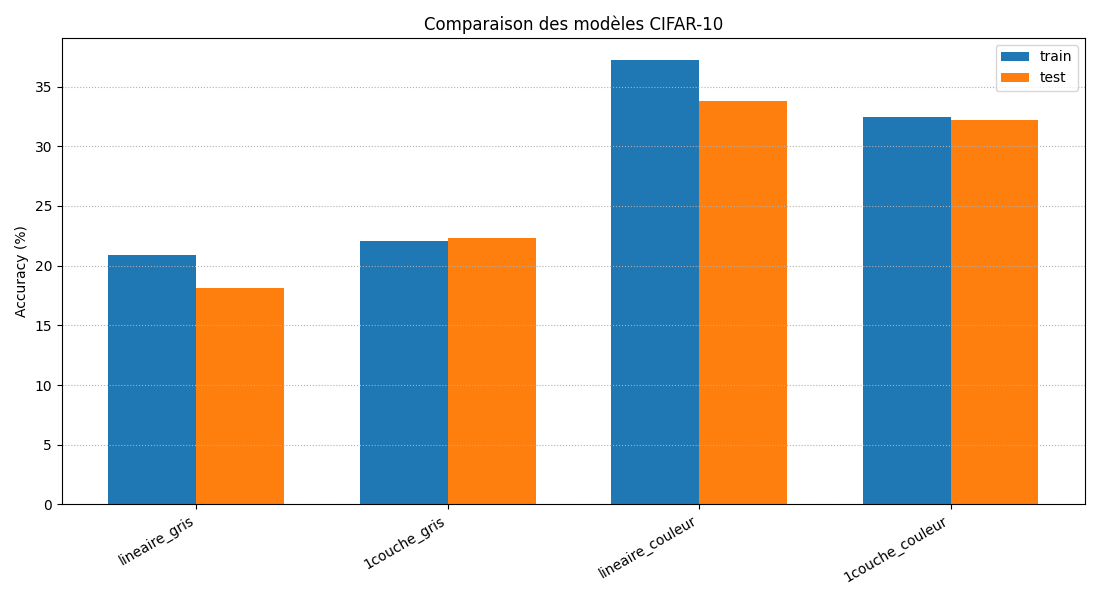
\includegraphics[width=\linewidth]{results/cifar10/model_comparison.png}
\caption{Comparaison des 5 modèles (train vs test).}
\end{subfigure}\hfill
\begin{subfigure}{0.49\textwidth}
\centering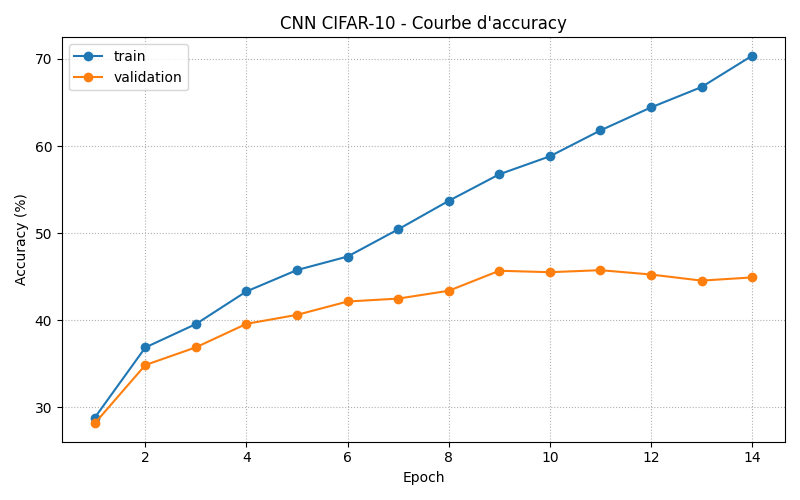
\includegraphics[width=\linewidth]{results/cifar10/accuracy_curve.png}
\caption{CNN : accuracy train vs validation (overfitting).}
\end{subfigure}
\caption{Résultats CIFAR-10.}
\label{fig:cifar}
\end{figure}

% ====================================================================
\section{CBIS-DDSM --- Détection de cancers du sein}
% ====================================================================
\textbf{Objectif et données.} Classification binaire de mammographies :
\textsc{Malignant} (malin, 1) contre \textsc{Benign}/\textsc{Benign\_without\_callback} (bénin, 0).
Nous utilisons les \textbf{vraies données} CBIS-DDSM (version JPEG). Les étiquettes proviennent de la
colonne \texttt{pathology} des CSV ; le \emph{matching} image\,$\leftrightarrow$\,label se fait via
\texttt{dicom\_info.csv} (vues « full mammogram »). Les images (jusqu'à $\sim\!4000\times3000$ px) sont
redimensionnées en $128\times128$ et normalisées. On charge \textbf{2\,857 vues} issues de
\textbf{1\,460 patients}.

\textbf{Déséquilibre.} $\sim\!44\%$ de malins dans le train : on utilise une \emph{weighted loss}
$\mathrm{BCEWithLogits}$ avec $\mathrm{pos\_weight}=n_{\text{bénin}}/n_{\text{malin}}\approx 1{,}26$.

\textbf{Architecture.}
$\mathrm{Conv}(1\!\to\!32)\!\to\!\mathrm{Conv}(32\!\to\!64)\!\to\!\mathrm{Conv}(64\!\to\!64)$
(chacune ReLU + MaxPool) $\to\!\mathrm{Flatten}\!\to\!\mathrm{Dense}(128)\!\to\!\mathrm{Dense}(1)$.
Adam ($10^{-3}$), early stopping (patience 5) sur la loss de validation.

Split \emph{officiel} CBIS-DDSM (CSV \texttt{*\_train}/\texttt{*\_test})
et validation découpée \emph{par patient} (aucun patient partagé). Les métriques chutent alors à des
valeurs réalistes (Tab.~\ref{tab:cbis}) --- c'est le résultat honnête.

\begin{table}[H]
\centering\small
\begin{minipage}{0.46\textwidth}\centering
\begin{tabular}{lc}
\toprule
Métrique & Valeur \\
\midrule
Accuracy & 0,602 \\
Précision & 0,512 \\
Rappel (sensibilité) & 0,634 \\
F1-score & 0,567 \\
ROC-AUC & \textbf{0,658} \\
\bottomrule
\end{tabular}
\end{minipage}\hfill
\begin{minipage}{0.50\textwidth}\centering
\begin{tabular}{lcc}
\toprule
 & Préd. bénin & Préd. malin \\
\midrule
Vrai bénin & 136 (VN) & 99 (FP) \\
Vrai malin & 60 (FN) & 104 (VP) \\
\bottomrule
\end{tabular}
\end{minipage}
\caption{CBIS-DDSM : métriques et matrice de confusion (test, 399 vues, split officiel par patient).}
\label{tab:cbis}
\end{table}

\vspace{-0.25cm}
\textbf{Analyse médicale.} Les \textbf{60 faux négatifs} ($\approx 37\%$ des malins) sont l'erreur la
plus grave : un cancer manqué retarde la prise en charge et engage le pronostic vital. Les
\textbf{99 faux positifs} entraînent des examens inutiles et de l'anxiété, mais ne sont pas dangereux.
En dépistage on privilégie donc un fort \emph{rappel}, quitte à accepter plus de faux positifs ; la
pondération \texttt{pos\_weight} et le seuil de décision (lisible sur la courbe ROC,
Fig.~\ref{fig:cbis}) permettent d'ajuster ce compromis. En l'état, ce taux de faux négatifs montre que
le modèle \textbf{n'est pas utilisable en clinique}.

\textbf{Limites.} CNN simple sans transfer learning ni augmentation ; résolution $128\times128$
(perte des micro-calcifications) ; mammographies complètes plutôt que patchs de lésions (ROI) ; un
seul split. La littérature atteint AUC $0{,}75$--$0{,}85$ avec des réseaux pré-entraînés et des ROI.

\begin{figure}[H]
\centering
\begin{subfigure}{0.40\textwidth}
\centering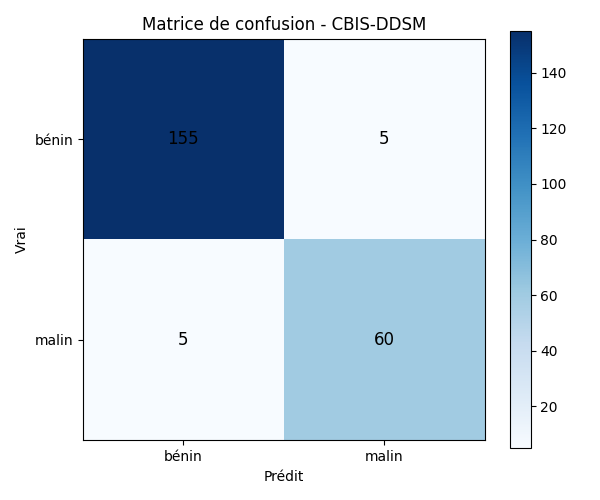
\includegraphics[width=\linewidth]{results/cbis_ddsm/confusion_matrix.png}
\caption{Matrice de confusion.}
\end{subfigure}\hspace{0.04\textwidth}
\begin{subfigure}{0.40\textwidth}
\centering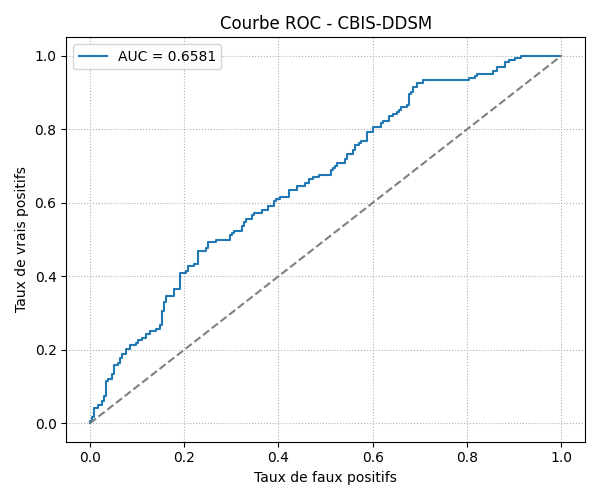
\includegraphics[width=\linewidth]{results/cbis_ddsm/roc_curve.png}
\caption{Courbe ROC (AUC $=0{,}658$).}
\end{subfigure}
\caption{Résultats du CNN sur CBIS-DDSM (données réelles, split par patient).}
\label{fig:cbis}
\end{figure}

% ====================================================================
\section*{Conclusion}
% ====================================================================
La difficulté croît nettement de MNIST ($\sim\!2{,}4\%$ d'erreur) à CIFAR-10 ($\sim\!54\%$) puis à
CBIS-DDSM (AUC $0{,}66$), à mesure que les images deviennent naturelles, variables et cliniquement
subtiles. Le CNN tire parti de la structure spatiale et de l'économie de paramètres, mais reste limité
sans techniques avancées. Le principal enseignement méthodologique est la \emph{fuite de données} :
un score « trop beau » doit alerter ; un protocole d'évaluation rigoureux (séparation par patient,
validation distincte du test) est indispensable, surtout en contexte médical.

% ====================================================================
\appendix
\section{Récapitulatif des taux d'erreur}
% ====================================================================
\begin{table}[H]
\centering\small
\begin{tabular}{llcc}
\toprule
Partie & Modèle & Err. train & Err. test \\
\midrule
MNIST & Linéaire & 8,19\,\% & 8,77\,\% \\
 & 1 couche (ReLU) & 0,66\,\% & 2,43\,\% \\
 & 2 couches (ReLU) & 1,29\,\% & 2,61\,\% \\
\midrule
CIFAR-10 & Linéaire (gris) & 79,7\,\% & 82,3\,\% \\
 & 1 couche (gris) & 62,4\,\% & 65,2\,\% \\
 & Linéaire (couleur) & 62,8\,\% & 65,9\,\% \\
 & 1 couche (couleur) & 50,2\,\% & 56,1\,\% \\
 & CNN (PyTorch) & 38,2\,\% & 54,0\,\% \\
\midrule
CBIS-DDSM & CNN binaire & 39,8\,\% & 39,8\,\% (acc. 60,2\,\%) \\
\bottomrule
\end{tabular}
\caption{Synthèse (taux d'erreur $=100-\text{accuracy}$).}
\end{table}

% ====================================================================
\section{MNIST --- Étude du learning rate (Conseil du professeur)}
% ====================================================================
\begin{table}[H]
\centering\small
\begin{tabular}{lccc}
\toprule
$\eta$ & Linéaire & 1 couche & 2 couches \\
\midrule
0,0001 & 19,90\,\% & 42,06\,\% & 88,58\,\% \\
0,0005 & 14,92\,\% & 15,18\,\% & 88,58\,\% \\
0,001  & 13,26\,\% & 12,90\,\% & 28,46\,\% \\
0,005  & 11,72\,\% & 8,68\,\% & 7,76\,\% \\
\textbf{0,01} & \textbf{11,62\,\%} & \textbf{7,74\,\%} & \textbf{6,88\,\%} \\
0,05   & 13,72\,\% & 8,96\,\% & 13,72\,\% \\
0,1    & 15,10\,\% & 20,96\,\% & 90,80\,\% \\
\bottomrule
\end{tabular}
\caption{Taux d'erreur test selon $\eta$ (10\,000 images, 5 epochs).}
\label{tab:lr}
\end{table}

\begin{figure}[H]
\centering
\begin{subfigure}{0.48\textwidth}
\centering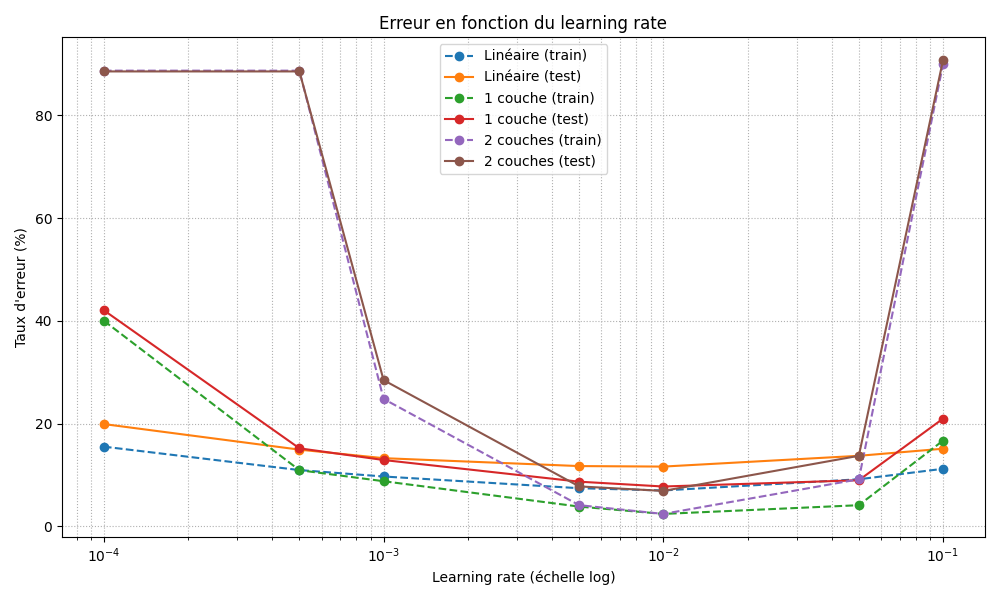
\includegraphics[width=\linewidth]{results/mnist/error_vs_learning_rate.png}
\caption{Erreur train/test vs $\eta$ (échelle log).}
\end{subfigure}\hfill
\begin{subfigure}{0.48\textwidth}
\centering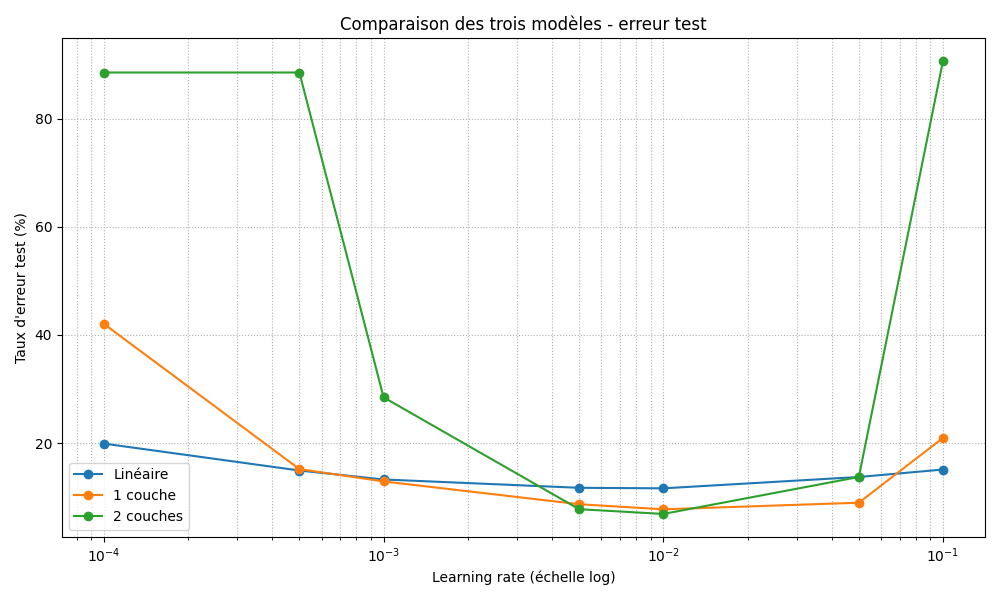
\includegraphics[width=\linewidth]{results/mnist/learning_rate_comparison.png}
\caption{Comparaison des trois modèles (erreur test).}
\end{subfigure}
\caption{Influence du learning rate sur les architectures MNIST.}
\label{fig:lr}
\end{figure}

% ====================================================================
\section{Courbes d'entraînement complémentaires}
% ====================================================================
\begin{figure}[H]
\centering
\begin{subfigure}{0.32\textwidth}
\centering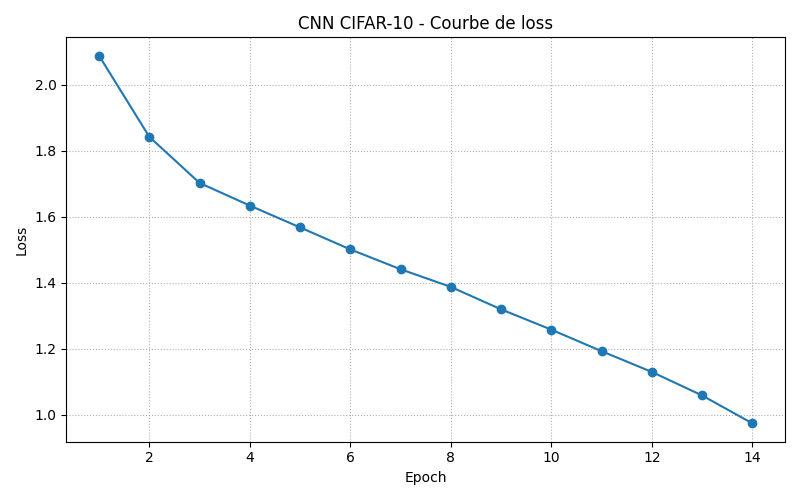
\includegraphics[width=\linewidth]{results/cifar10/loss_curve.png}
\caption{CIFAR-10 : loss CNN.}
\end{subfigure}\hfill
\begin{subfigure}{0.32\textwidth}
\centering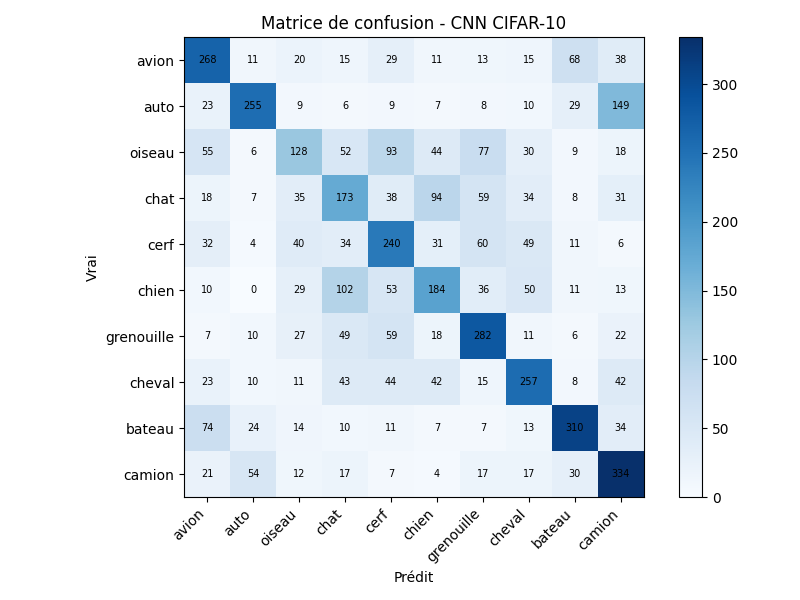
\includegraphics[width=\linewidth]{results/cifar10/confusion_matrix.png}
\caption{CIFAR-10 : confusion CNN.}
\end{subfigure}\hfill
\begin{subfigure}{0.32\textwidth}
\centering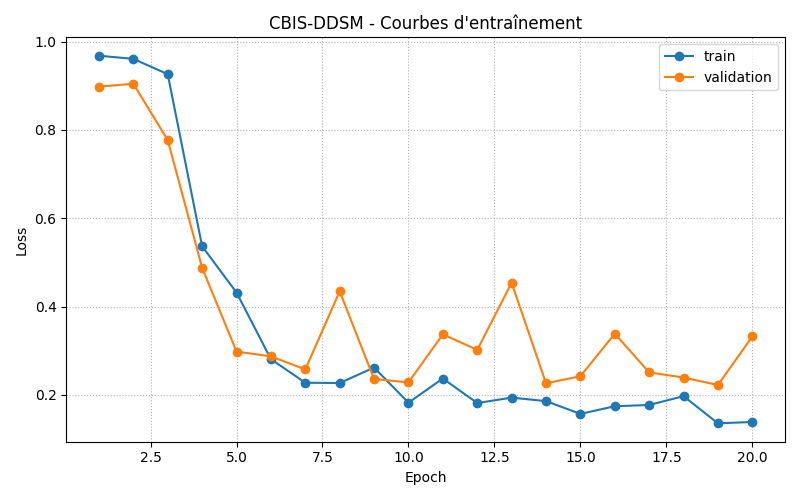
\includegraphics[width=\linewidth]{results/cbis_ddsm/training_curves.png}
\caption{CBIS-DDSM : loss train/val.}
\end{subfigure}
\caption{Courbes complémentaires. La matrice de confusion CIFAR-10 met en évidence les confusions
inter-classes attendues (chat/chien, auto/camion, cerf/cheval).}
\end{figure}

\end{document}
